%% Cao's Paper
%% March 2018
%%%%%%%%%%%%%%%%%%%%%%%%%%%%%%%%%%%%%%%%%%%%%%%%%%%%%%%%%%%%%%%%%%%%%%%%%%%%
% AGUJournalTemplate.tex: this template file is for articles formatted with LaTeX
%
% given in the order necessary to produce a final output that will
% satisfy AGU requirements, including customized APA reference formatting.
%
% You may copy this file and give it your
% article name, and enter your text.
%
%
% Step 1: Set the \documentclass
%
% There are two options for article format:
%
% PLEASE USE THE DRAFT OPTION TO SUBMIT YOUR PAPERS.
% The draft option produces double spaced output.
%

%% To submit your paper:
\documentclass[draft,linenumbers]{agujournal2019}
\usepackage{apacite}
\usepackage{url} %this package should fix any errors with URLs in refs.
\usepackage{natbib}

%%%%%%%
% As of 2018 we recommend use of the TrackChanges package to mark revisions.
% The trackchanges package adds five new LaTeX commands:
%
%  \note[editor]{The note}
%  \annote[editor]{Text to annotate}{The note}
%  \add[editor]{Text to add}
%  \remove[editor]{Text to remove}
%  \change[editor]{Text to remove}{Text to add}
%
% complete documentation is here: http://trackchanges.sourceforge.net/
%%%%%%%

\draftfalse

%% Enter journal name below.
%% Choose from this list of Journals:
%
% JGR: Atmospheres
% JGR: Biogeosciences
% JGR: Earth Surface
% JGR: Oceans
% JGR: Planets
% JGR: Solid Earth
% JGR: Space Physics
% Global Biogeochemical Cycles
% Geophysical Research Letters
% Paleoceanography and Paleoclimatology
% Radio Science
% Reviews of Geophysics
% Tectonics
% Space Weather
% Water Resources Research
% Geochemistry, Geophysics, Geosystems
% Journal of Advances in Modeling Earth Systems (JAMES)
% Earth's Future
% Earth and Space Science
% Geohealth
%
% ie, \journalname{Water Resources Research}

\journalname{JGR: Atmospheres}


\begin{document}

%% ------------------------------------------------------------------------ %%
%  Title
%
% (A title should be specific, informative, and brief. Use
% abbreviations only if they are defined in the abstract. Titles that
% start with general keywords then specific terms are optimized in
% searches)
%
%% ------------------------------------------------------------------------ %%

% Example: \title{This is a test title}

\title{Simulating the transportation and dispersal of volcanic ash cloud with initial condition created by 3D plume model}
% \title{Effect on dispersal of vertical distribution of pyroclasts in plume: 3D plume simulations as source for long-range transport and dispersal models}

%% ------------------------------------------------------------------------ %%
%
%  AUTHORS AND AFFILIATIONS
%
%% ------------------------------------------------------------------------ %%

% Authors are individuals who have significantly contributed to the
% research and preparation of the article. Group authors are allowed, if
% each author in the group is separately identified in an appendix.)

% List authors by first name or initial followed by last name and
% separated by commas. Use \affil{} to number affiliations, and
% \thanks{} for author notes.
% Additional author notes should be indicated with \thanks{} (for
% example, for current addresses).

% Example: \authors{A. B. Author\affil{1}\thanks{Current address, Antartica}, B. C. Author\affil{2,3}, and D. E.
% Author\affil{3,4}\thanks{Also funded by Monsanto.}}


% \affiliation{1}{First Affiliation}
% \affiliation{2}{Second Affiliation}
% \affiliation{3}{Third Affiliation}
% \affiliation{4}{Fourth Affiliation}

%\affiliation{=number=}{=Affiliation Address=}

%(repeat as many times as is necessary)

%% Corresponding Author:
% Corresponding author mailing address and e-mail address:

% (include name and email addresses of the corresponding author.  More
% than one corresponding author is allowed in this LaTeX file and for
% publication; but only one corresponding author is allowed in our
% editorial system.)

% Example: \correspondingauthor{First and Last Name}{email@address.edu}

\correspondingauthor{Abani Patra}{abani.uftspatra@t.edu}

%% Keypoints, final entry on title page.

%  List up to three key points (at least one is required)
%  Key Points summarize the main points and conclusions of the article
%  Each must be 100 characters or less with no special characters or punctuation

% Example:
% \begin{keypoints}
% \item	List up to three key points (at least one is required)
% \item	Key Points summarize the main points and conclusions of the article
% \item	Each must be 100 characters or less with no special characters or punctuation
% \end{keypoints}

\begin{keypoints}
 \item Creating initial conditions for volcanic ash transport and dispersal models based on 3D plume model output eliminates need for assumptions or inversion regarding initial ash particle distribution with height, and improves prediction capability.
\item Initial particle distribution in vertical direction has greater impact on transport of ash clouds than does horizontal distribution.
\item Ash particles involved in long-range transport are initially concentrated in the umbrella cloud of large eruptions.
\end{keypoints}

%% ------------------------------------------------------------------------ %%
%
%  ABSTRACT
%
% A good abstract will begin with a short description of the problem
% being addressed, briefly describe the new data or analyses, then
% briefly states the main conclusion(s) and how they are supported and
% uncertainties.
%% ------------------------------------------------------------------------ %%

%% \begin{abstract} starts the second page

\begin{abstract}
 VATDs (volcanic ash transportation and dispersion) model atmospheric transport of ash starting from a source originating at the volcano represented by concentrations of ash with height.  Most VATD models use a line source of some prescribed shape calibrated against an empirical expression for the height-mass eruption rate (MER) relation.  Such empirical vertical ash distributions are often inadequate representations of actual vertical ash distributions, which usually vary from case to case and have complex dependencies on eruption source parameters and atmospheric conditions.  We present here for the first time the use of 3D (three-dimensional) plume models  to represent ash cloud source without any assumption regarding plume geometry. By eliminating assumed behavior associated with the semiempirical plume geometry, the predictive skill of VATD simulations are greatly improved. 
 To date no VATD simulation adopt initial condition created from first principles based 3D plume simulation. We use our recently developed volcanic plume model based on a 3D Lagrangian method [Cao et al, Geophysical Model Dev., 2018] and couple the output to a standard Lagrangian VATD model and apply to historical eruptions to illustrate the effectiveness of this approach.  The importance of the source model is shown in sensitivity analyses which prove that volcanic ash transportation simulation is much more sensitive to the source geometry than all other input parameters. Further investigation also reveals that initial particle distribution in vertical direction has more mpact on transportation of ash clouds than horizontal distribution. Comparison also indicates that ash particles are concentrated along intrusion height of umbrella cloud that is much lower than the plume top, which is just momentum overshoot.
\end{abstract}

%% ------------------------------------------------------------------------ %%
%
%  PLAIN LANGUAGE SUMMARY
%
% This is optional but will help expand the reach of your paper.
% Information on writing a good plain language summary is available at:
% http://sharingscience.agu.org/creating-plain-language-summary/
%
% If your paper doesn't include a Plain Language Summary, remove the
% commands below.
%% ------------------------------------------------------------------------ %%

%\begin{plainlanguage}
%All exising VATD (volcanic ash transport and dispersion) simulations are initialized by either a cylindrical source or a specified ash distribution depending on the context. This paper proposes a new way to create initial conditions for VATD simulation based on 3D (three dimensional) numerical model of volcanic plume. Without any semiempirical expressions, the new method eliminates parameters calibration and hence user intervention associated with the semiempirical expressions. Therefore, predict capability of VATD simulation can be improved if adopt initial condition created based on this new method.
%\end{plainlanguage}


%% ------------------------------------------------------------------------ %%
%
%  TEXT
%
%% ------------------------------------------------------------------------ %%

\section{Introduction}

\subsection{Volcanic Ash Transportation Forecast}
The fine-grain fraction of tephra (volcanic ash) can be widely dispersed, and can lead to a degradation of air quality and pose threats to aviation \citep{tupper2007facing}. Identification of volcanic ash helps schedule flights to avoid areas where ash is present. Numerical estimation of ash distribution using known and forecast wind fields is necessary if we are to accurately predict ash cloud evolution. Numerous VATD (volcanic ash transportation and dispersion) models have been developed by both civil and military aviation or meteorological agencies to provide forecasts of ash cloud motion \citep{witham2007comparison}. New techniques have been integrated with VATDs to satisfy increasing demands for more outputs, model accuracy and forecast reliability. This contribution explores a method for creating initial conditions for VATD simulations, which promises to improve prediction capability and accuracy.

\citet{fero2009simulating, stohl2011determination} showed that initial source conditions have significant effects on simulation of volcanic ash transportation.  Traditional VATD simulation requires key global descriptors of the volcanic plumes, especially plume height, grain size, eruption duration and mass loading, or alternatively, a mass eruption rate (MER). No matter how these global descriptors are obtained, they are used to furnish the initial conditions for VATDs in the form of a line-source term of a spatio-temporal distribution of particle mass. It is a common practice to pick values for these global descriptors using an empirical expression for the height-MER relation. The empirical expression is written as a function of several parameters, including the key global descriptors.  The values for the descriptors can also be found by parameter calibration \citep[e.g.][]{fero2008simulation,fero2009simulating, stohl2011determination, zidikheri2017estimation}. 1D plume models serve as an alternative option to provide values. For example, \citet{bursik2012estimation} and \citet{stefanescu2014temporal} used the 1D model puffin \citep{bursik2001effect} to generate estimates of mass eruption rate and grain size.  In some cases, an extra step is adopted to spread ash particles from the line source horizontally, resulting in an initial ash cloud in 3D space.  The horizontal spreading depends on an empirical expression. For example, the VATD model Puff spreads particles from the line source uniformly in the horizontal direction within a given radius using an empirical expression in puffin.  Considering the complexities of volcanic eruptions, the actual ash distribution in initial ash clouds should vary from case to case and with time, making it difficult to find one general expression that is suitable for all cases. It is useful therefore to investigate alternative ways for creating initial ash clouds without assumptions regarding plume geometry or numerical inversion. This provides the  major motivation of this paper.

\subsection{Numerical Tools}
VATD models can be categorized into Lagrangian particle tracking and Eulerian advection-diffusion types.  Among several available particle tracking models \citep[e.g.][]{walko1995hypact, searcy1998puff, d1998modeling, draxler1998overview} and advection-diffusion models \citep[e.g.][]{bonadonna2005total, folch2009fall3d, schwaiger2012ash3d}, we adopt a particle tracking model, Puff \citep{tanaka1991development,searcy1998puff}, as the VATD model. Puff can take 3D ash clouds as initial conditions, which makes it technically easier to couple with 3D plume models. Puff initializes a discrete number of tracers that represent a sample of the eruption cloud, and calculates transport, turbulent dispersion, and fallout for each representative tracer.  A cylinder emanating vertically from the volcano summit to a specified maximum height is the standard approach to provide a simple model of the geometry of a typical ash column. Puff minimally requires horizontal wind field data. The ``restart feature'' of Puff makes it technically feasible to accommodate the hand-off between a plume simulation and the Puff simulation in terms of time and length scales.

Besides parameter calibration, 1D (one dimensional) plume models have been used to obtain global descriptors of volcanic plumes.  1D plume models \citep [e.g.][]{woods1988fluid, bursik2001effect, mastin2007user, de2015plume, folch2016fplume, pouget2016sensitivity} solve the equations of motion in 1D using simplifying assumptions, and hence depend on estimation of certain parameters, especially those related to the entrainment of air, which is evaluated based on two coefficients: a coefficient due to turbulence in the rising buoyant jet, and one due to the crosswind field. Different 1D models adopt different entrainment coefficients based on a specific formulation or calibration against well-documented case studies. The feedback from plume to atmosphere is usually ignored in 1D models. While these 1D models generated well-matched results with 3D models for plumes that are  dominated by wind (often called weak plumes) much greater variability is observed for strong plume scenarios \citep{costa2016results}. On the other hand, 3D numerical models for volcanic plumes based on first principles and having few parametrized coefficients \citep{oberhuber1998volcanic, neri2003multiparticle, suzuki2005numerical, cerminara2016ashee, cao2018plume} naturally create a 3D ash cloud, which could serve directly as an initial state of the volcanic material for VATDs. However, there is no VATD simulation using such 3D ash clouds as initial conditions. In this paper, we will carry out VATD simulations using an initial state for the ash cloud based on 3D plume simulations, generated with Plume-SPH \citep{cao2018plume}.  The implementation techniques described in this paper can be applied for any combination of VATD model and 3D plume model even though our investigation is based on a specific VATD model and plume model.

\subsection{Pinatubo Eruption}

The 1991 eruption of Pinatubo volcano is used as a case study.  Pinatubo erupted between June 12 and 16, 1991, after weeks of precursory activity. The climactic phase started on June 15 at 0441 UTC and ended around 1341 UTC \citep{holasek1996satellite}. The climactic phase generated voluminous pyroclastic flows, and sent Plinian and co-ignimbrite ash and gas columns to great altitudes \citep{scott1996pyroclastic}. The evolution of the Pinatubo ash and $SO_2$ clouds was tracked using visible \citep{holasek1996satellite}, ultraviolet (Total Ozone Mapping Spectrometer; TOMS) \citep{guo2004re} and infrared sensors, including the Advanced Very High-Resolution Radiometer (AVHRR) \citep{guo2004particles}. There are also sufficient observational data to estimate the eruption conditions for the climactic phase of the eruption \citep{suzuki2009three}. The availability of calibrated eruption conditions and extensive observational data regarding ash clouds transport make the Pinatubo eruption an ideal case study.

\section{Setting up Simulations} \label{sec:Methodology}

\subsection{Creation of Initial Ash Cloud} \label{sec:create-initial-condition}

\begin{figure}
\center
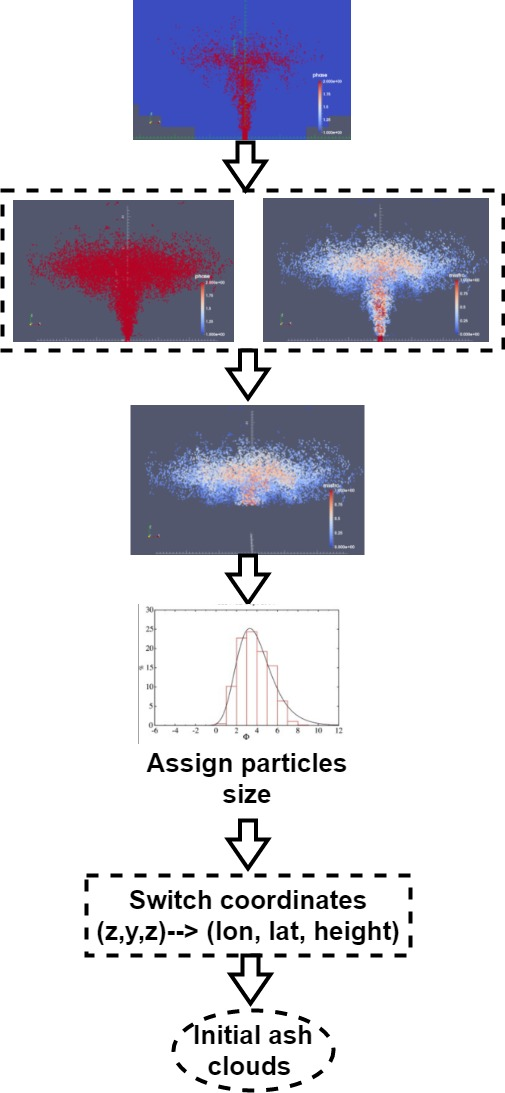
\includegraphics[width=0.43\textwidth]{Figures/Creat_initial_Ash}
\caption{Work flow to create initial condition for Puff based on raw output of Plume-SPH. Top:  raw output of Plume-SPH. Blue particles are phase 1 (ambient air), red particles are  phase 2 (erupted material).  Second row: plume after removing SPH particles of phase 1. Left: colored according to mass fraction of erupted material. Third row:  volcanic plume above the ``corner'' region after cutting off lower portion.}
\label{fig:create-initial-ash-plume-sph}
\end{figure}

The steps to create an initial ash cloud based on the raw output of Plume-SPH are shown in Fig. \ref{fig:create-initial-ash-plume-sph}.
The method proposed consists in generating the initial ash cloud directly from Plume-SPH, foregoing  assumptions and estimates or  inverse modeling regarding ash injection height and timing thereof.
We use Plume-SPH as an example, noting that for other 3D plume models, the steps would be similar. Plume-SPH is a two-phase model based on the Lagrangian smoothed-particle hydrodynamics (SPH) method, in which the computational domain is discretized by SPH particles. The current version, Plume-SPH 1.0 \citep{cao2018plume}, uses two types of SPH particles: 1) particles of phase 1 to represent ambient air, and 2) particles of phase 2 to represent erupted material. The initial ash cloud is created from SPH particles of phase 2.

After reaching the maximum rise height and starting to spread horizontally, particles of phase 2 form an initial umbrella cloud (Fig. \ref{fig:Plume-SPH-Pinatubo-ash-cloud}). The 3D plume simulation is considered complete once the umbrella cloud begins to form. Parcels that will be transported by the ambient wind are those above the ``corner'' region, where mean plume motion is horizontal rather than vertical.  

Considering that SPH particles are only discretization points, each is assigned a grain size according to a given total grain size distribution (TGSD) \citep{paladio1996tephra}, and a concentration according to the mass and volumetric eruption rate. The Plume-SPH discretization points are thus switched to Puff Lagrangian tracer particles having grain sizes and concentrations. The coordinates of these tracer particles, which are initially in the local Cartesian coordinate system of Plume-SPH, are converted into Puff's global coordinate system, which is given in terms of $(longitude, latitude, height)$. Puff takes the initial ash cloud, consisting of the collection of Lagrangian tracer particles with grain size and concentration, and propagates from time $t$ to time $t+\Delta t$ via an advection/diffusion equation \citep{searcy1998puff}.
\begin{linenomath*}
\begin{equation}
\textbf{R}_i(t+\Delta t) = \textbf{R}_i(t) + \textbf{W}(t)\Delta t + \textbf{Z}(t)\Delta t +  \textbf{S}_i(t) \Delta t
\end{equation}
\end{linenomath*}
Here, $\textbf{R}_i(t)$ is the position vector of the $i^{th}$ Lagrangian tracer particle at time $t$, $\textbf{W}$ accounts for wind advection, $\textbf{Z}$ accounts for turbulent dispersion and $\textbf{S}$ is the terminal gravitational fallout velocity, which depends on tracer's size.

To summarize, there are four steps to create an initial ash cloud from the raw output of Plume-SPH:
\begin{enumerate}
\item filter by SPH particle type to select SPH particles that represent erupted material (phase 2)
\item filter by a mean velocity threshold to select the upper part (above the ``corner'' region) dominated by horizontal transport
\item switch SPH discretization points to Lagrangian tracer particles, by assigning grain size to each particle
\item convert coordinates of the SPH Lagrangian tracers into the VATDs' geographic coordinate system
\end{enumerate}
The features of the volcanic plume and resulting initial ash cloud used in the case study are shown in Fig. \ref{fig:Plume-SPH-Pinatubo-ash-cloud}. It is important to point out that since both Plume-SPH and Puff are based on the Lagrangian method, there is no extra step of conversion between an Eulerian grid and Lagrangian particles.

\begin{figure}[!htb]
    \centering
    \begin{minipage}{.325\textwidth}
        \centering
        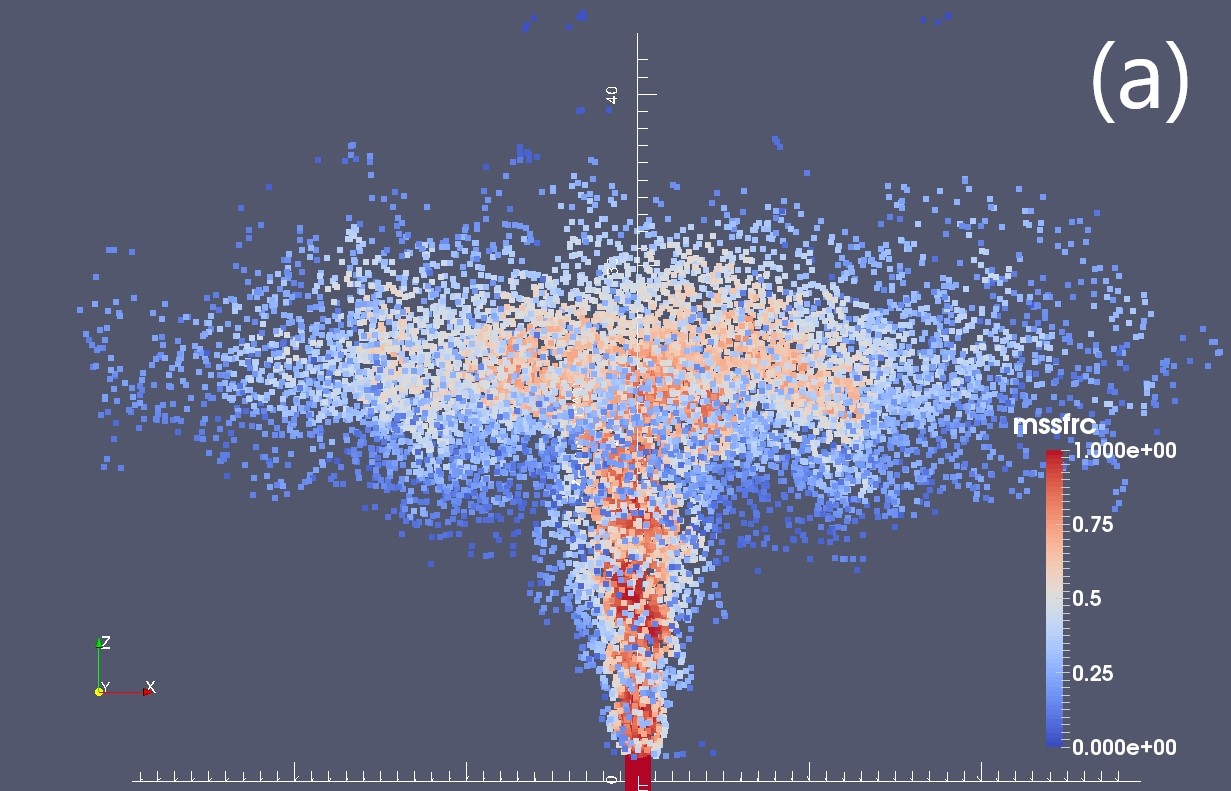
\includegraphics[width=0.99 \textwidth]{Figures/mssfrc_front-filter-by-phase}
    \end{minipage}%
    \begin{minipage}{.325 \textwidth}
        \centering
        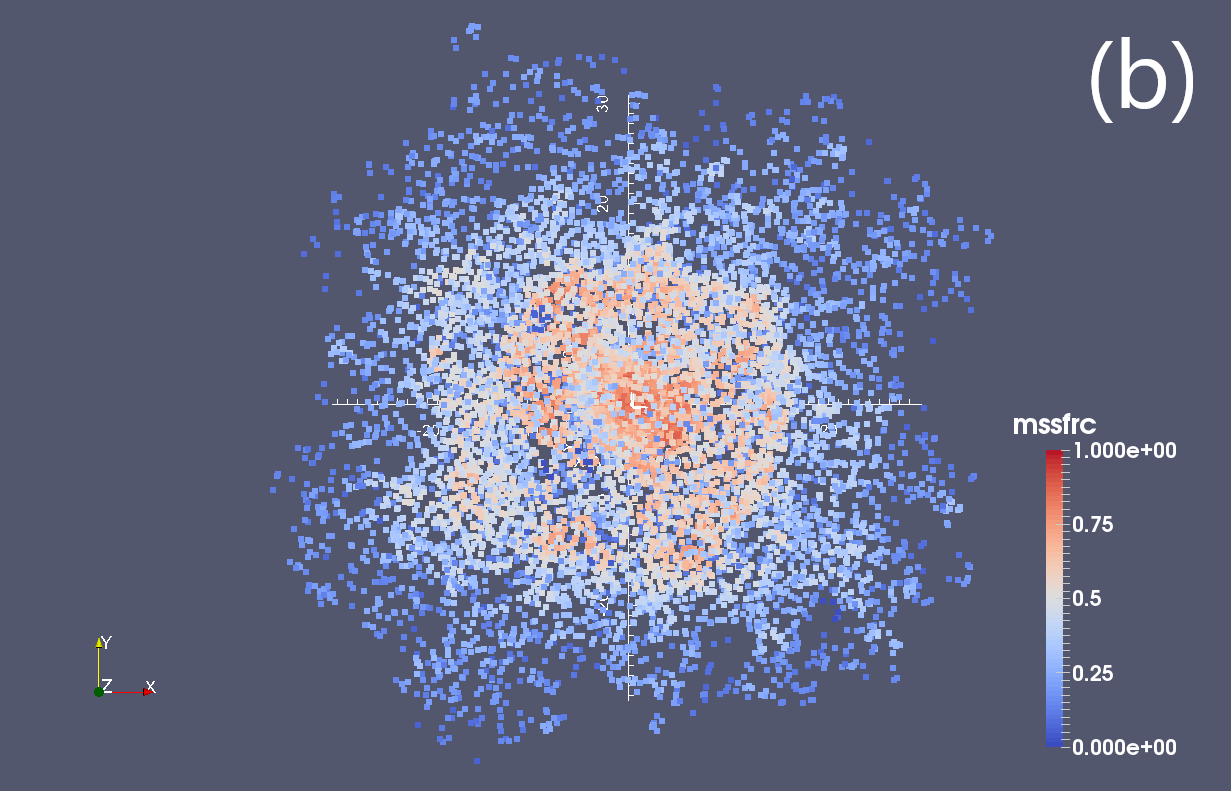
\includegraphics[width=0.99 \textwidth]{Figures/mssfrc_top-with-axis}
    \end{minipage}%
    \begin{minipage}{.325 \textwidth}
        \centering
        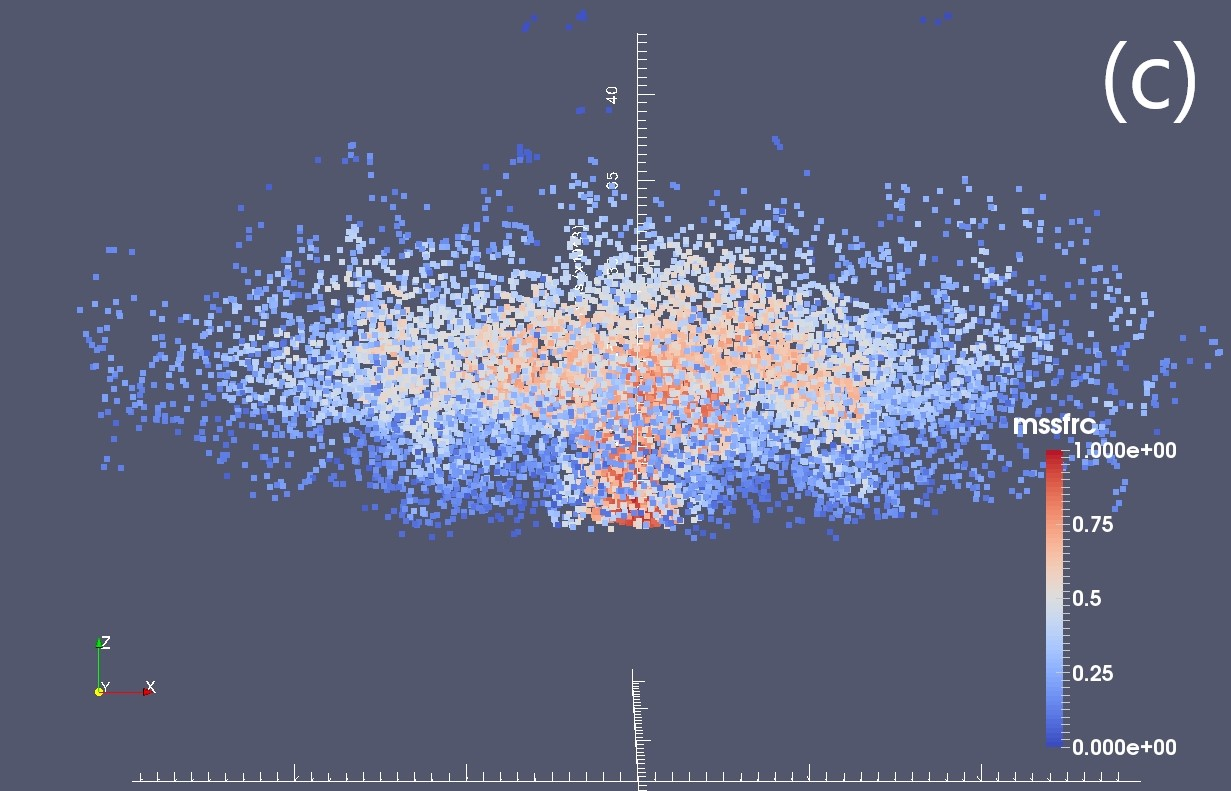
\includegraphics[width=0.99 \textwidth]{Figures/mssfrc_front-z15000}
    \end{minipage}%   
    \caption{All particles in the pictures are of type phase 2 (phase 1 has been removed in step 1) at $600s$ after eruption, at which time, the plume has already reached the maximum height and started spreading radially. Pictures from left to right are: front view of the whole plume, top view of the plume and front view of the initial ash cloud, which is essentially portion of the whole plume with elevation higher than a given threshold (in this picture is $15000 m$). Particles are colored according to mass fraction of erupted material. Red represents high mass fraction while blue represents low mass fraction.}
    \label{fig:Plume-SPH-Pinatubo-ash-cloud}
\end{figure}

Table \ref{tab:VATDs-source-term-determination} compares three different methods for creating initial conditions for VATD simulation: 1) creating initial condition based on parameter calibration without any plume model (method 1), 2) creating initial condition based on output of 1D plume model (method 2), 3) extracting initial ash cloud from 3D plume simulation (method 3). The first method determines all global descriptors of volcanic plume based on calibration. Then create initial line source or ash cloud according to semiempirical plume shape expression. Both other two methods depend on plume models. However 3D plume models can generate initial ash cloud in 3D space while 1D plume models only obtain global descriptors of plume so still need semiempirical expression to create 3D initial ash cloud. In addition, the number of Lagrangian tracers is a free parameter when using semiempirical plume shape expressions while it purely depends on simulation when creating initial condition from 3D plume simulation results.

\begin{table}
\centering
      \caption{Three different methods for creating initial conditions (initial ash clouds) for Puff simulation}		
	  \begin{tabular}{p{26.5mm}p{25.5mm}p{36.5mm}p{34.5mm}}
	    \hline
	    		 & No model & 1D model & 3D model \\
	    		 \hline    		 
	  Maximum height & Calibration & Semiempirical &  1st principle \\
	  Average height &  Calibration & Conservation laws (1D) &  1st principle  \\
	  Vertical spread &  Calibration & Semiempirical & 1st principle \\
	  Column radius & Calibration  &  Conservation laws (1D) &  1st principle \\
	  Plume shape & Semiempirical & Semiempirical  & 1st principle \\
	  Tracers number & Free parameter  & Free Parameter & Based on simulation\\ 
	    \hline
	  \end{tabular}
	  \label{tab:VATDs-source-term-determination}
\end{table}

\subsection{Puff Restart}

The plume and ash transport models are run at different time scales and length scales.  The spatial and temporal resolutions of the plume simulations are much finer than those of the ash transport model. It takes tens of minutes ($600 s$ in this case) for the Pinatubo plume to reach a steady height. However the eruption persisted for a few hours (9 hours for the climactic phase of Pinatubo eruption), and it may be necessary to track ash transport for days following an eruption.  At present, it is too expensive computationally to do 3D plume simulations of several hours in real time. In order to handle the difference in time scale, we mimic a continuing eruption with intermittent pulsed releasing of ash particles. Particularly, we restart Puff at an interval of $600 s$, i.e., the physical time of the plume simulation to reach steady height. At every Puff restart, we integrate the output of the last Puff simulation and Plume-SPH into a new ash cloud. This new ash cloud serves as a new initial condition with which to restart a Puff simulation. The interval of the pulsed releases is the simulation time of Plume-SPH, i.e., $600 s$ in our case study. A sketch demonstrating the overall restart process is shown in Fig. (\ref{fig:Restart-Puff}). The total number of Lagrangian tracer particless used in Puff thus equals the summed number of particles in all releases. So the total number of tracer particles is no longer a user-selected parameter.  \citet{fero2008simulation} proposed using more realistic time-dependent plume heights. We do not adopt that strategy here for simplicity, although the idea would be straightforward in execution.

\begin{figure}
\center
\includegraphics[width=0.90 \textwidth]{Figures/Restart-Puff.pdf} 
    \caption{Mimic successive eruption with intermittent pulsing releasing of ash particles. $t_I$ is the period of pulsing release. $t_I$ equals to physical time of 3D plume simulation.}
    \label{fig:Restart-Puff}
\end{figure}

\subsection{Sensitivity Analysis of Other Parameters}

Besides the positions of particles in the initial ash cloud, other parameters for Puff simulations are: horizontal diffusivity, vertical diffusivity, mean grain size, grain size standard deviation and total number of tracers. We present in this subsection systematic sensitivity studies on these parameters. We also investigate the influence of eruption duration.  The sensitivity analyses will serve as the basis for identifying possible sources of disparities between simulation and observation.

The sensitivity analyses illustrate that adjustment of other parameters produces negligible visual differences in VATD simulation results. Using different vertical diffusivities in range of $[100, 100000] m^2s^{-1} $ and different horizontal diffusivities in range of $[1, 20] m^2s^{-1}$ produces visually negligible differences.  The simulation eruption duration should depend on the total observed duration or the duration of the climactic phase. We conducted several simulations with eruption duration varying in range of $[5, 11] hours$ with slight different starting time of climactic phase. Table \ref{tab:Pinatubo-eruption-duration} lists all these simulations. However, only tiny visible differences are observed among the simulated ash transportation. The mean of grain size also has visually ignorable effects on long-term ash transportation according to our sensitivity tests varying the log mean (base 10) grain radius in a range of $[-7.3, -3.5] m$.  The standard deviation, when varying in range of $[0.1, 10]$, generate ignorable difference on long-term ash transportation as well. Similar conclusion on parameter sensitivity is reported by \citet[e.g.][]{fero2008simulation, daniele2009applications}.  Among these parameters, the eruption duration and beginning time shows, even though tiny, the most obvious influence on simulated ash distribution. In order to show such differences in an intuitive way, Fig. \ref{tab:Pinatubo-eruption-duration} shows simulated ash distribution corresponding to 4.9 hours duration, 9 hours duration and 11 hours duration respectively. After 72 hours, relative to the simulation starting time, these three cases generate generally similar results, with high concentration ash covers almost the same region. The difference of lower concentration distribution is relatively more obvious. Ash cloud covers broadest area when eruption duration is 11.1 hours. To summarize, all these parameters have either tiny or ignorable affects on long-term ash distribution simulation.

\begin{table}[htp]
\centering
      \caption{The starting and ending time (UT) for simulating the climactic phase of Pinatubo eruption on June 15 1991. Observed plume height \citep{holasek1996satellite} at different time are also list in the table.}		
	  \begin{tabular}{p{35mm}p{20mm}p{20mm}p{20mm}p{20mm}}
	    \hline
        Eruption duration & 4.9 hours & 9 hours & 10 hours & 11.1 hours \\
	    \hline
	    Start time & 0441 & 0441 & 0441 & 0334 \\
	    Height at start time & 37.5 km & 37.5 km  & 37.5 km  & 24.5 km \\
	    
	    End time   & 0934 & 1341 & 1441 & 1441  \\
	    	Height at end time & 35 km & 26.5 km & 22.5 & 22.5 km \\
	    \hline
	  \end{tabular}
	  \label{tab:Pinatubo-eruption-duration}
\end{table}

\begin{figure}[!htb]
    \centering
    \begin{minipage}{.325\textwidth}
        \centering
        \includegraphics[width=0.99 \textwidth]{Figures/199106180441-ash-5hr-cut15000}
    \end{minipage}%
    \begin{minipage}{.325 \textwidth}
        \centering
        \includegraphics[width=0.99 \textwidth]{Figures/199106180441-ash-9hr-cut15000}
    \end{minipage}%
    \begin{minipage}{.325 \textwidth}
        \centering
        \includegraphics[width=0.99 \textwidth]{Figures/199106180441-ash-11hr-cut15000}
    \end{minipage}%   
    \caption{Simulated ash cloud distribution corresponding to eruption duration of 4.9 hours, 9 hours and 11.1 hours (from left to right) respectively. Starting and ending time for each case is in Table \ref{tab:VATDs-source-term-determination}. The contours are for ash distribution at 72 hours after eruption.}
    \label{fig:Puff-sensitivity-duration}
\end{figure}

The new methodology for generating initial ash cloud introduces another new parameter: elevation threshold. We also carry out sensitivity analysis on this parameter by varying the elevation threshold from $1500 m$ (the height of the vent) to $25000 m$. The simulated ash distributions show obviously visible differences. Such influence is especially obvious when the elevation threshold is either very large or very small. However, varying the elevation threshold in the range of $[12000, 18000] m$ generates relatively small difference in ash transportation simulation results. Figure \ref{fig:Puff-sensitivity-elevation-threshold} compares the simulated ash distribution corresponding to elevation thresholds of $1500 m$ and $15000 m$. Compared with ash distribution for threshold of $15000 m$, an extra long tail appears when using elevation threshold of $1500 m$. Adopting smaller elevation thresholds essentially adds more tracers at lower elevation. As the wind at different elevations are different, these tracers at lower elevation would transpose to different directions. The forward trajectories, which starting at June 15 1624 UTC, indicates that the wind between evaluation 10000 m to 15000 m blows from north-east to south-west while wind of higher evaluation blows from east to west. 

\begin{figure}[!htb]
    \centering
    \begin{minipage}{.325\textwidth}
        \centering
        \includegraphics[width=0.99 \textwidth]{Figures/199106180441-ash-9hr-cut1500}
    \end{minipage}%
    \begin{minipage}{.325 \textwidth}
        \centering
        \includegraphics[width=0.99 \textwidth]{Figures/199106180441-ash-9hr-cut15000}
    \end{minipage}%
    \caption{Simulated ash distribution taking initial ash clouds obtained using different elevation thresholds ($1500 m$ and $15000$ m) from output of Plume-SPH. The contours are corresponding to ash concentration at 72 hours after eruption. The starting and ending time are corresponding to 9 hours duration case in Table \ref{tab:Pinatubo-eruption-duration}}
    \label{fig:Puff-sensitivity-elevation-threshold}
\end{figure}

\begin{figure}[!htb]
    \centering
    \begin{minipage}{.75 \textwidth}
        \centering
        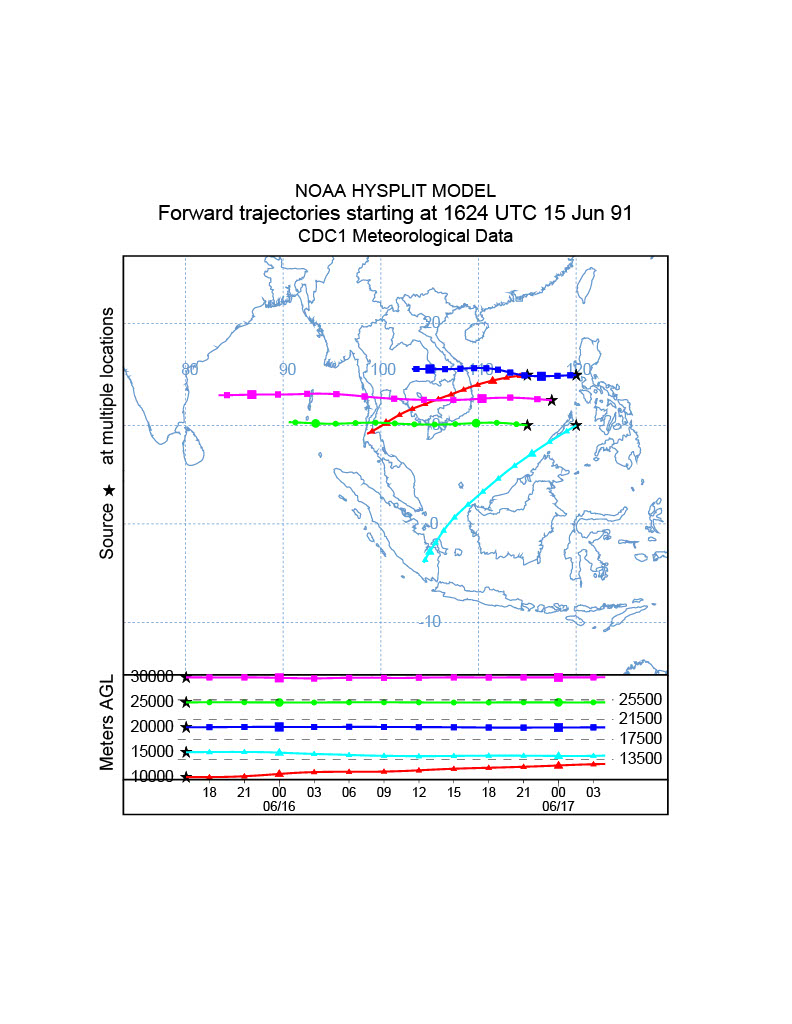
\includegraphics[width=0.99 \textwidth]{Figures/trajplot_test3_10_30K_ok}
    \end{minipage}%   
    \caption{Trajectories of particles starting from different heights indicating the wind direction of different evaluations.}
    \label{fig:hysplit-1624-utc}
\end{figure}

The sensitivity analyses demonstrate that the initial condition for VATD simulation has the most significant effect on simulated ash distribution while all other input parameters have either tiny or ignorable influence. The initial ash cloud generated based on semiempirical expression, which is a function of several parameters, might be significantly disparate from realistic ash cloud. Such initial condition might greatly compromise the accuracy of VATDs simulation.


In this paper, we do not carry out any investigation with respect to wind field even though it is another dominant factor in VATD simulation. In the case study, we use global $NOAA/OAR/ESRL 6-h, 2.0^{\circ}$ reanalysis wind fields data \citep{whitaker2004reanalysis, compo2006feasibility, compo2011twentieth}.

\section{Comparison and Discussion}

Transportation of volcanic ash resulted from Pinatubo eruption on June 15th 1991 is simulated using two different initial conditions.
The initial condition is created in traditional way according to key global descriptors and semiempirical plume shape expression. The second initial condition is created by the new method proposed in this paper.  Simulated ash transportation results are compared against observation. 

\begin{table}[htp]
	\centering
      \caption{List of eruption condition and material properties for plume simulation}		
	  \begin{tabular}{lrr}
	    \hline
	    Parameters & Units & Plume \\
	    \hline
	    Vent velocity          & $m\cdot s^{-1}$  & 275 \\
	    Vent gas mass fraction &                  & 0.05 \\
	    Vent Temperature       & $K$              & 1053 \\
	    Vent height            & $m$              & 1500 \\
	    Mass discharge rate    & $kg\cdot s^{-1}$ & $1.5 \times 10^9$\\
	    	Specific heat of gas at constant volume     & $J \cdot kg^{-1}\cdot K^{-1}$ & 717     \\
	    Specific heat of air at constant volume     & $J \cdot kg^{-1}\cdot K^{-1}$ & 1340    \\
	    	Specific heat of solid                      & $J \cdot kg^{-1}\cdot K^{-1}$ & 1100    \\
	    	Specific heat of gas at constant pressure   & $J \cdot kg^{-1}\cdot K^{-1}$ & 1000    \\
	    	Specific heat of air at constant pressure   & $J \cdot kg^{-1}\cdot K^{-1}$ & 1810    \\
	    	Density of air at vent height               & $kg \cdot m^{-3}$       & 1.104   \\
	    Pressure at vent height                     & $Pa$                    & 84363.4 \\
	    \hline
	  \end{tabular}
	  \label{tab:input_parameters_plume_simulation}
\end{table}

To create initial condition using the new method described in this paper, the plume rise  is simulated first by Plume-SPH. The eruption parameters, material properties and atmosphere for the strong plume no wind case in a comparison study on eruptive column models \citep {costa2016results} are adopted. Eruption conditions and material properties are listed in Table \ref{tab:input_parameters_plume_simulation}. Note that the density of erupted material at the vent and radius of the vent can be computed from the given parameters. The eruption pressure is assumed to be the same as pressure of ambient at the vent and hence is not given in the table. The vertical profiles of atmospheric properties were obtained based on the reanalysis data from ECMWF (European Centre for Medium-Range Weather Forecasts) for the period corresponding to the climactic phase of the Pinatubo eruption. The initial ash cloud is obtained by processing the raw output of Plume-SPH following steps described in Sec. \ref{sec:Methodology}.

Another set of initial condition is created based on observed top height ($40 km$) and several other parameters assigned semiempirically \citep{bursik2012estimation}. These parameters, namely, the global descriptors of volcanic plume, are used as parameters of semiempirical expression to get ash cloud in 3D space. See details in Table \ref{tab:input_parameter_Puff_simulation}. Except for initial condition, the simulation parameters that control VATD simulation are the same for both simulations. As has been shown in sensitivity analyses section, these parameters have less influence on simulation results than initial condition.
 
\begin{table}[htp]
\centering
      \caption{Parameters used in VATD simulation of the climactic phase of Pinatubo eruption on June 15 1991. The first six parameters are used by semiempirical expression to create initial ash cloud. When create initial condition based on Plume-SPH model, these parameters are extracted from output of Plume-SPH model.}
	  \begin{tabular}{lrrr}
	    \hline
	    Parameters & Unit & Semiempirical & Plume-SPH \\
	    \hline
	    Maximum Height ($H_{max}$) & $m$ & 40000 & 41800 \\
	    Horizontal Spread ($R_{max}$) & $km$ & 103.808 & -\\
	    Vertical Spread ($H_{width}$) & $km$ & 6.662  & - \\
	    Plume Shape & - & Poisson & - \\
	    Total Ash Particles  & - & 1768500 & 1768500 \\
	    Elevation Threshold & $m$ & - &  15000 \\
	    Horizontal Diffusivity & $m^2/s$ &10000 & 10000\\
	    Vertical Diffusivity & $m^2/s$ & 10 & 10 \\
	    Grain Size Distribution & - & Gaussian & Gaussian  \\
	    Mean of Grain Size (Radius) & $mm$ & $3.5 \times 10 ^-2$ & $3.5 \times 10 ^-2$ \\
	    Standard Deviation of Grain Size & - &  1.0 & 1.0 \\
	    	Start Time & UT & 0441 & 0441 \\
	    End time & UT & 1341 & 1341 \\
	    Simulation Duration & hour & 72 & 72 \\
	    \hline
	  \end{tabular}
	  \label{tab:input_parameter_Puff_simulation}
\end{table}

\subsection{``Plume-SPH + Puff" and ``Semiempirical Initial Cloud + Puff"}

The simulation results using different initial conditions are compared with TOMS images and AVHRR BTD ash cloud map in Fig. \ref{fig:Plume-SPH-Puff-ash-cloud}.

\begin{figure}[!htb]
    \centering
    \begin{minipage}{.325\textwidth}
        \centering
        \includegraphics[width=0.99 \textwidth]{Figures/bent-23hr-ash}
    \end{minipage}%
    \begin{minipage}{.325 \textwidth}
        \centering
        \includegraphics[width=0.99 \textwidth]{Figures/SPH-Plume-23hr-ash}
    \end{minipage}%
    \begin{minipage}{.325 \textwidth}
        \centering
        \includegraphics[width=0.99 \textwidth]{Figures/OB-ash-23hr-ash}
    \end{minipage}% 
    \\
        \begin{minipage}{.325\textwidth}
        \centering
        \includegraphics[width=0.99 \textwidth]{Figures/bent-31hr-ash}
    \end{minipage}%
    \begin{minipage}{.325 \textwidth}
        \centering
        \includegraphics[width=0.99 \textwidth]{Figures/SPH-Plume-31hr-ash}
    \end{minipage}%
    \begin{minipage}{.325 \textwidth}
        \centering
        \includegraphics[width=0.99 \textwidth]{Figures/OB-ash-31hr-ash}
    \end{minipage}% 
    \\
        \begin{minipage}{.325\textwidth}
        \centering
        \includegraphics[width=0.99 \textwidth]{Figures/bent-55hr-ash}
    \end{minipage}%
    \begin{minipage}{.325 \textwidth}
        \centering
        \includegraphics[width=0.99 \textwidth]{Figures/SPH-Plume-55hr-ash}
    \end{minipage}%
    \begin{minipage}{.325 \textwidth}
        \centering
        \includegraphics[width=0.99 \textwidth]{Figures/OB-ash-55hr-ash}
    \end{minipage}% 
    \caption{Comparison between ``Semiempirical initial cloud + Puff" and ``Plume-SPH + Puff". Pictures from left to right are: Puff simulation based on initial condition created according to semiempirical plume shape expression, Puff simulation based on initial condition generated by Plume-SPH, TOMS or AVHRR image of Pinatubo ash cloud. Ash clouds at different hours after eruption are on different rows. From top to bottom, the images are corresponding to around 23 hours after eruption (UT 199106160341), 31 hours after eruption (UT 199106161141), 55 hours after eruption (UT 199106171141). The observation data on the first row are TOMS ash and ice map. The observation data on the second and third row are AVHRR BTD ash cloud map with atmospheric correction method applied \citep{guo2004particles}.}
    \label{fig:Plume-SPH-Puff-ash-cloud}
\end{figure}

The differences between simulated ash transportation by ``Semiempirical initial cloud +Puff" and ``Plume-SPH+Puff" are obvious. The simulated ash concentration based on initial condition created from Plume-SPH is much closer to observation than that based on semiempirical plume shape expression. Around 23 hours and 31 hours after the beginning of the climactic phase, ``Plume-SPH + Puff" simulation generates ash images that generally close to observational image, especially the location where high concentration ash presents. However, these ash at near west to Pinatubo mountain observed in satellite images does not show up in ``Plume-SPH + Puff" simulation results. This disparity is very possible due to the fact that the Mountain Pinatubo continued erupting after climactic phase while our simulation only simulates the climactic phase. The ash released after climactic phase is not accounted in our simulation results. The ``Semiempirical initial cloud + Puff" simulation, however, forecasts an ash distribution faster and narrower than observation. The location, where the high concentration ash presents, locates to the far northwest of observed ash. 
Around 55 hours after the beginning of the climactic phase, the disparity between observation and simulation becomes more obvious. Ash distribution of ``Semiempirical initial cloud + Puff" simulation locates far west to the observed ash. The high concentration area of ``Plume-SPH + Puff" simulation, even though closer to observation than that of ``Semiempirical initial cloud +Puff", is still faster than observation.

Except for the initial condition, both simulations adopt the same parameters and wind field data. That is to say, the only difference between these two simulations is the initial condition. Recall that the initial condition has most significant influence on ash transportation simulation. It is therefore very likely that the big difference between simulation results by ``Plume-SPH+Puff" and ``Semiempirical initial cloud +Puff" may be attributed to the initial condition and thereby be credited with its added skill.% The ash transportation simulation based on 3D plume simulation results is much more accurate than that based on semiempirical initial cloud.

\subsection{Discussion Regarding Maximum Height ($H_{max}$)}

In this section, we mainly discuss the vertical distribution of ash particles in initial ash cloud.
The majority of volcanic ash particles usually present a lower elevation than maximum height. For instance, \citet{holasek1996satellite, holasek1996experiments} reported the maximum Pinatubo plume height as high as around $39 km$ while the cloud heights were estimated at $20 \sim 25 km $, \citet{self1993atmospheric} report the maximum plume height could be $>35 km$ and the plume heights are $23 \sim 28 km$ after $15 \sim 16$ hours. The neutral buoyant regions of the Pinatubo aerosol estimated by different measurements are: $17 \sim 26 km$ (lidar) by \citet{defoor1992early}, $20 \sim 23 km$ (balloon) by \citet{deshler1992balloonborne}, $17 \sim 28 km$ (lidar) by \citet{jager1992pinatubo}, and $17 \sim 25 km$ (lidar) by \citet{avdyushin19931}. Based on comparison between simulated cloud with early infrared satellite images of Pinatubo, \citet{fero2008simulation} reported that the majority of ash was transported between $16 km$ and $18 km$. This is physically understandable as particles are concentrated along intrusion height of umbrella cloud, not near top because the plume top is due to momentum overshoot. However, the empirical expressions for the height-MER relation, which are commonly adopted to create initial conditions for VATD simulation, tends to place majority of ash particles closer to top if use observed maximum height in the empirical expressions.

Here we check two commonly used plume shapes, the Poisson and Suzuki.
For Poisson plume shape, the vertical height of ash particles are determined according to Eq. (\ref{eq:Poisson-plume-shape}).
\begin{equation}
H=H_{max} - 0.5 H_{width}*P+H_{width}R
\label{eq:Poisson-plume-shape}
\end{equation}
where $P$ is an integral value drawn from a Poisson distribution of unit mean, $R$ is a uniformly distributed random number between 0 and 1, $H_{max}$ is the maximum plume height, $H_{width}$ represents an approximate vertical range over which the ash will be distributed.
For Suzuki plume shape \citep{suzuki1983theoretical}, volcano ash mass vertical distribution is assumed to follow the Suzuki equation (Eq. (\ref{eq:Suzuki-plume-shape})).
\begin{equation}
Q(z)=Q_m* \frac{k^2(1-z/H_{max})exp\left(k(z/H_{max} -1 )\right)}{H_{max}\left[1-(1+k)exp(-k)\right]}
\label{eq:Suzuki-plume-shape}
\end{equation}
Where $Q_m$ is the total mass of erupted material, $k$ is shape factor, which is an adjustable constant that controls ash distribution with height. A low value of $k$ gives a roughly uniform distribution of mass with elevation, while high values of $k$ concentrate mass near the plume top.

Particle distribution (in terms of mass percentage or particle number percentage) in vertical direction in the initial ash cloud are shown in Fig. \ref{fig:Particle-distribution-Plume-SPH-vs-semiempirical}. In that figure, the vertical particle distribution based on Plume-SPH output is compared with vertical particle distribution created based on semiepirical shape expressions. Both Poisson and Suzuki distribution in Fig. \ref{fig:Particle-distribution-Plume-SPH-vs-semiempirical} take $H_{max} = 40000m$, which is close to reported observation of maximum height. When adopting Poisson plume shape, the majority of the particles are between $30 km \sim 40 km$. Obviously, Poisson distributes majority ash at a much higher elevation than observations \citep[e.g.][]{fero2008simulation}. As for Suzuki, the majority of ash particles also distribute in a range that significantly higher than $25 km$. As for initial ash cloud based on Plume-SPH simulation, the major population of ash particles distribute between $17 km \sim 28 km$, which match well with observations. The maximum height is also consistent with observation. To summarize, using semiempirical plume shape expression generates unrealistic initial ash cloud even if we use observed plume maximum height.

\begin{figure}[!htb]
    \centering
    \begin{minipage}{.247\textwidth}
        \centering
        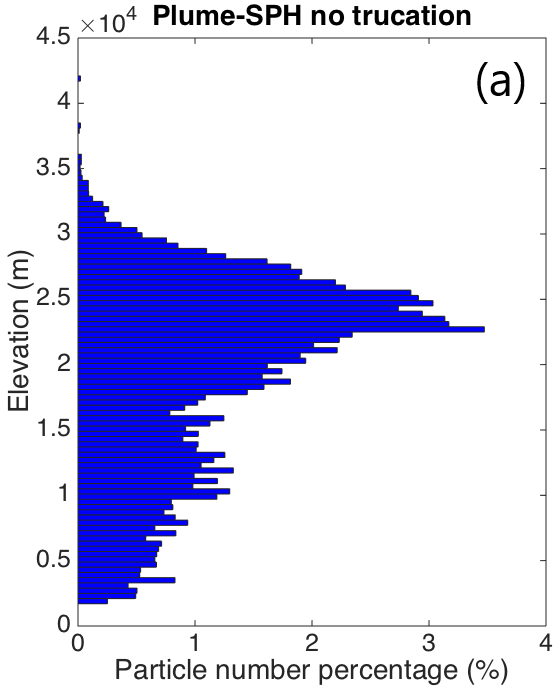
\includegraphics[width=0.99 \textwidth]{Figures/Plume-SPH-ParticleDis-NoTrucation-z}
    \end{minipage}%
    \begin{minipage}{.247 \textwidth}
        \centering
        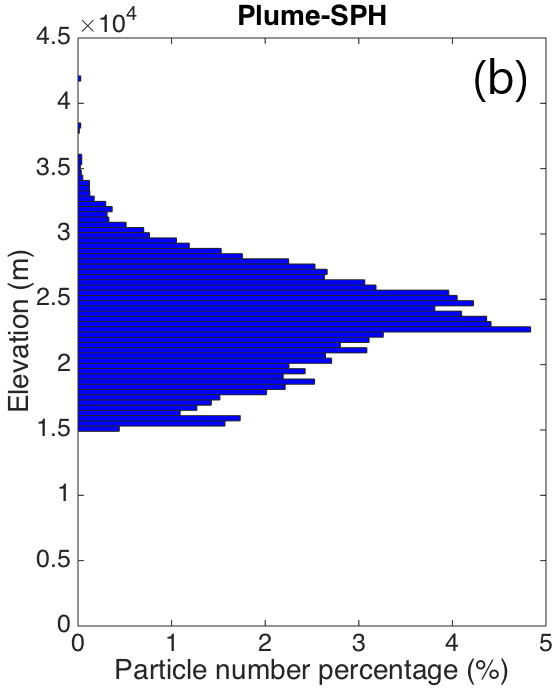
\includegraphics[width=0.99 \textwidth]{Figures/Plume-SPH-ParticleDis-z}
    \end{minipage}%
    \begin{minipage}{.247 \textwidth}
        \centering
        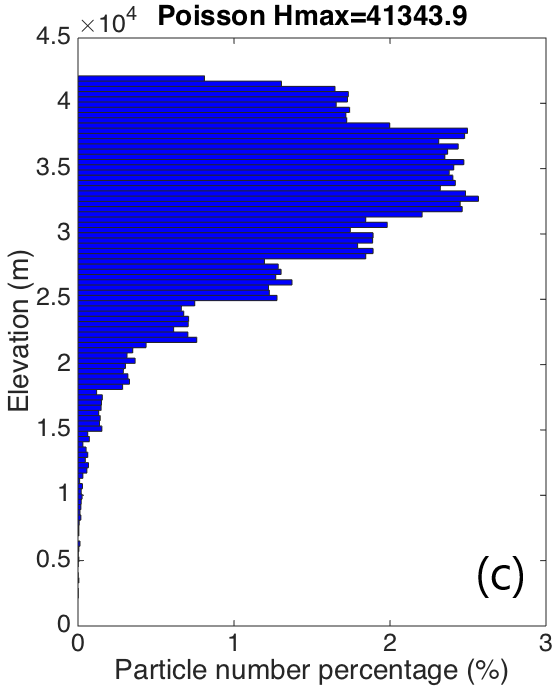
\includegraphics[width=0.99 \textwidth]{Figures/Possion-Hmax40k-ParticleDis-z}
    \end{minipage}% 
    \begin{minipage}{.247 \textwidth}
        \centering
        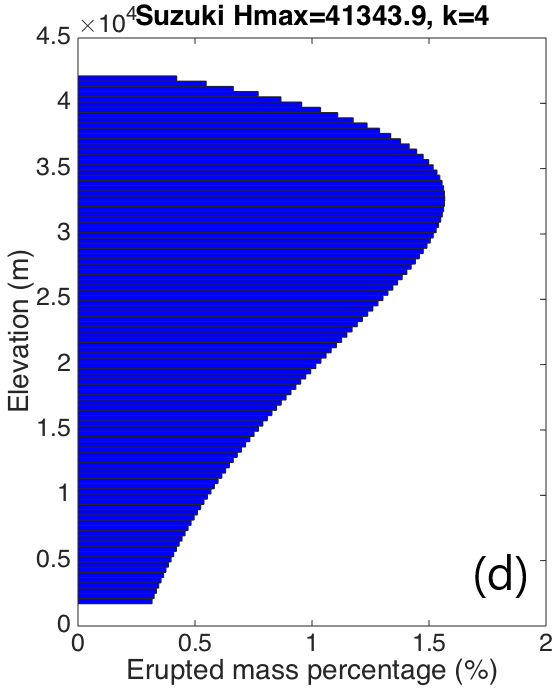
\includegraphics[width=0.99 \textwidth]{Figures/Suzuki-Hmax40k-ParticleDis-z}
    \end{minipage}% 
    \caption{Particle distribution of initial ash cloud in vertical direction. The picture to the left is corresponding to initial ash cloud obtained from Plume-SPH output. The second picture is corresponding to ash distribution truncated by a elevation threshold of $15000 m$. The third picture is for vertical ash distribution based on Poisson distribution with maximum height equals to $40000 m$. Another parameter, the vertical spread, in the expression of Poisson plume shape is $6662 m$. The picture to the right is corresponding to Suzuki distribution with maximum height equals to $40000 m$. Another parameter in Suzuki distribution, the shape factor, is $4$. The $x$ axis is the percentage of particle number for Plume-SPH and Poisson. For Suzuki the $x$ axis is the mass percentage of erupted material.}
    \label{fig:Particle-distribution-Plume-SPH-vs-semiempirical}
\end{figure}

For Poisson and Suzuki plume shape, vertical distribution of ash particles can't be lower down without changing the maximum height. To distribute major population of ash particles at lower elevation, the maximum height has to be reduced to a value smaller than observed maximum height. Adjusting parameters such as maximum height in the emperical expression is actually the traditional source term calibration method. A set of initial ash clouds using different maximum heights based on Poisson plume shape is shown in Fig. \ref{fig:Particle-distribution-Plume-calibrate-semiempirical}). The maximum heights adopted in plume shape expressions are, by no means, obtained from any plume model or observation. Except for maximum height, all other parameters for creating initial ash cloud are the same as these in Table \ref{tab:input_parameter_Puff_simulation}. The range, between which major populations of ash particles locate, is lower when using smaller maximum heights. These ash clouds created by Poisson distribution with different maximum heights are then used as initial condition in Puff simulation, whose results are show in Fig. \ref{fig:Various-Maximum-height-Pinatubo-ash-cloud}.

\begin{figure}[!htb]
    \centering
    \begin{minipage}{.247 \textwidth}
        \centering
        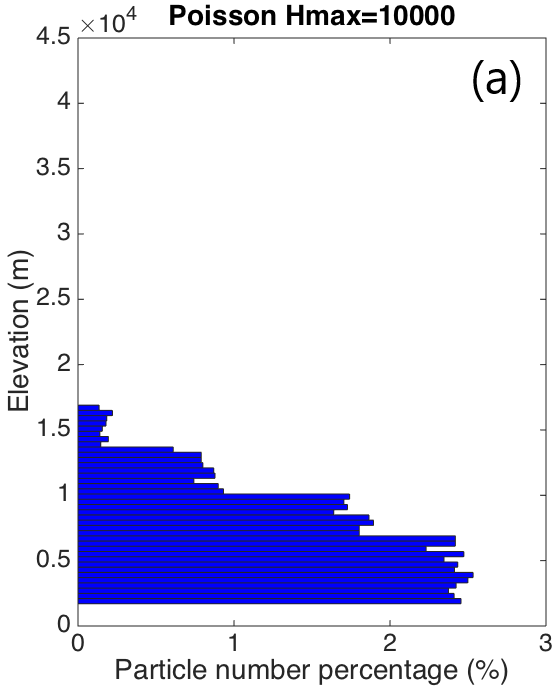
\includegraphics[width=0.99 \textwidth]{Figures/Possion-Hmax10k-ParticleDis-z}
    \end{minipage}%
    \begin{minipage}{.247 \textwidth}
        \centering
        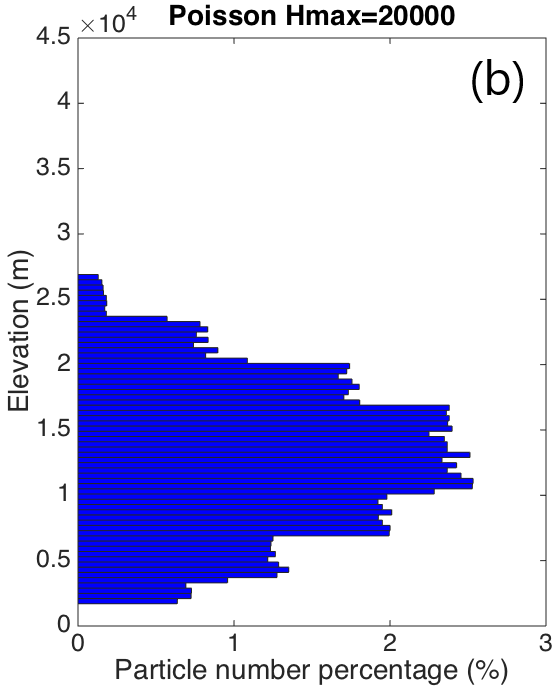
\includegraphics[width=0.99 \textwidth]{Figures/Possion-Hmax20k-ParticleDis-z}
    \end{minipage}% 
    \begin{minipage}{.247 \textwidth}
        \centering
        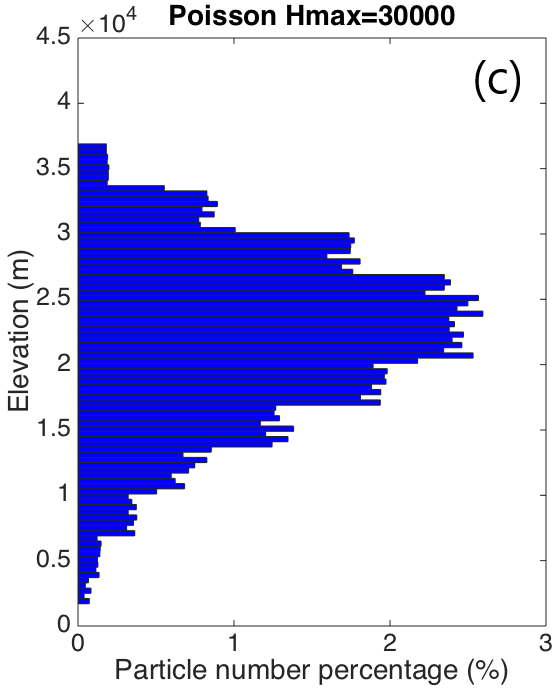
\includegraphics[width=0.99 \textwidth]{Figures/Possion-Hmax30k-ParticleDis-z}
    \end{minipage}% 
    \begin{minipage}{.247 \textwidth}
        \centering
        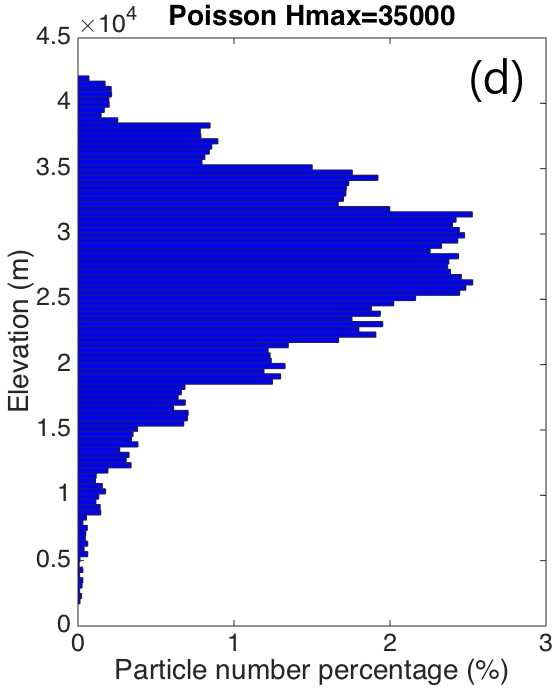
\includegraphics[width=0.99 \textwidth]{Figures/Possion-Hmax35k-ParticleDis-z}
    \end{minipage}% 
    \caption{Initial particle distribution in vertical direction based on Poisson plume shape with different maximum heights. Pictures from left to right are corresponding to maximum height of $10000 m$,  $20000 m$,  $30000 m$, $35000 m$. Another parameter, the vertical spread, in the expression of Poisson plume shape is $6662 m$ for all cases. The $x$ axis is the percentage of particle number. See Fig. \ref{fig:Particle-distribution-Plume-SPH-vs-semiempirical} for vertical ash distribution of Plume-SPH output.}
    \label{fig:Particle-distribution-Plume-calibrate-semiempirical}
\end{figure}

\begin{figure}[!htb]
    \centering
    \begin{minipage}{.245\textwidth}
        \centering
        \includegraphics[width=0.99 \textwidth]{Figures/bent-55hr-ash-MaxH10000}
    \end{minipage}%
    \begin{minipage}{.245 \textwidth}
        \centering
        \includegraphics[width=0.99 \textwidth]{Figures/bent-55hr-ash-MaxH20000}
    \end{minipage}%
    \begin{minipage}{.245 \textwidth}
        \centering
        \includegraphics[width=0.99 \textwidth]{Figures/bent-55hr-ash-MaxH30000}
    \end{minipage}%  
    \begin{minipage}{.245 \textwidth}
        \centering
        \includegraphics[width=0.99 \textwidth]{Figures/bent-55hr-ash-MaxH35000}
    \end{minipage}%   
    \caption{Ash transportation simulated by Puff using different initial ash cloud created according to Poisson distribution with different maximum heights. Pictures from left to right are corresponding to maximum plume heights of $10000 m$, $20000 m$, $30000 m$ and $35000 m$. All images are for simulated ash transportation around 55 hours after eruption (UT 199106171141). See the observed cloud image in Fig. \ref{fig:Plume-SPH-Puff-ash-cloud}.}
    \label{fig:Various-Maximum-height-Pinatubo-ash-cloud}
\end{figure}

Figure \ref{fig:Various-Maximum-height-Pinatubo-ash-cloud} shows that the maximum height has significant influence on ash transportation simulation. When the maximum height is $10000 m$ the high concentration area is lag behind observation. While the designated maximum height is $35000 m$, the high concentration area is a little bit faster and much narrower than observation. When using maximum height of $41343.9 m$, the high concentration area is faster and narrower than both observation and ``Pume-SPH+Puff" simulation results (see Fig. \ref{fig:Plume-SPH-Puff-ash-cloud}). The simulated high concentration area is closest to ``Pume-SPH+Puff" simulation results when assigning a maximum height of $30000 m$. The front of volcano ash, with lower concentration is faster than observation locating far west to high concentration area. A lower concentration tailing area also appears in the simulation results while there is no such tail in observed image. Puff simulation result based on calibrated maximum height of $30000 m$ shows similar footprint to, even though smaller in terms of covered area than, those of ``Pume-SPH+Puff" simulation. However, the initial ash cloud created by Poisson distribution with maximum height around  $20000 m$ generates best match ash distribution with observation. That is to say, a maximum height lower than real maximum height is required by Poisson plume shape to distribute ash particles at the same elevation as real ash distribution. This is physically understandable as maximum plume heights are reached due to overshoot. 
Our hypothesis regarding the sources of disparity between "Semiempirical initial cloud +Puff" simulation and observation is confirmed. Since the initial condition has so dominant an effect on VATD simulation, it is critical for the forecast capability of VATD simulation to explore the more accurate and adaptive ways for establishing the initial conditions, especially the method that does not rely on "post event" parameter calibration.

\subsection{Discussion Regarding Vertical Spread ($H_{width}$)}
In previous section, the maximum height is adjusted to change vertical ash distribution along the source line. This section investigates another parameter in semiempirical Poission expression. We vary the ``vertical spread" ($H_{width}$) in range $3 km /~ 10 km$. A set of initial ash clouds created according to different ``vertical spread" is shown in Fig. \ref{fig:poisson-vertical-spread}. Except for ``vertical spread", all other parameters for creating initial ash cloud are the same as these in Table \ref{tab:input_parameter_Puff_simulation}. Width of the range within which major populations of ash particles locate become narrower when a smaller value for vertical spread is used. But changing $H_{width}$ has no obvious affect on the height at which majority of ash particles distribute. These ash clouds based on different vertical spread are then used as initial condition in Puff simulation, whose results are show in Fig. \ref{fig:Various-vertical-spread-Pinatubo-ash-cloud}.

Adjusting of the vertical spread can change particle distribution in vertical direction and not surprisely affect VATD simulation results. Unluckily, none of these VATD simulations based on initial ash cloud with vertical spread equals to $3km$, $5km$, and $10 km$ get better results than VATD simulation based on initial condition created by a 3D plume simulation using Plume-SPH (see Fig. \ref{fig:Various-vertical-spread-Pinatubo-ash-cloud}).

\begin{figure}[!htb]
    \centering
    \begin{minipage}{.325 \textwidth}
        \centering
        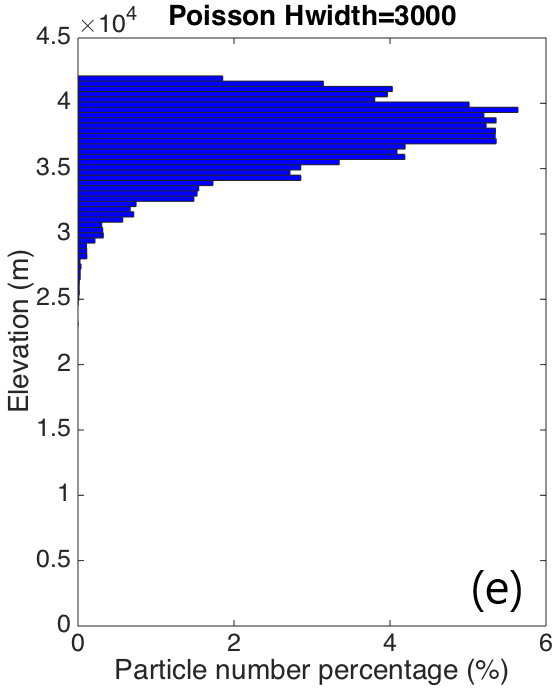
\includegraphics[width=0.99 \textwidth]{Figures/Possion-Hwidth3k-ParticleDis-z}
    \end{minipage}%
    \begin{minipage}{.325 \textwidth}
        \centering
        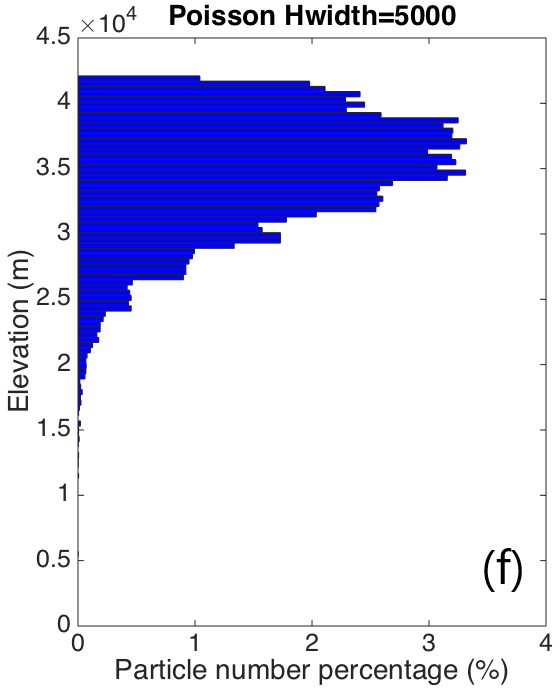
\includegraphics[width=0.99 \textwidth]{Figures/Possion-Hwidth5k-ParticleDis-z}
    \end{minipage}% 
    \begin{minipage}{.325 \textwidth}
        \centering
        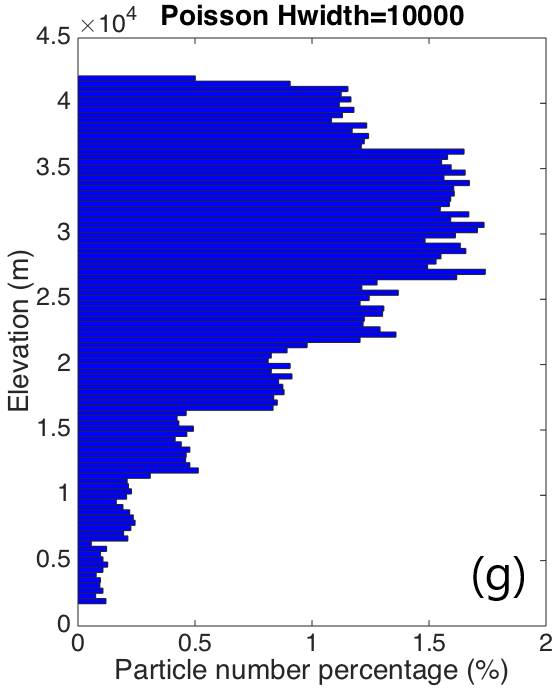
\includegraphics[width=0.99 \textwidth]{Figures/Possion-Hwidth10k-ParticleDis-z}
    \end{minipage}% 
    \caption{Vertical particle distribution based on Poisson plume shape with different ``vertical spread". Pictures from left to right are corresponding to vertical spread of $3km$, $5km$ and $10 km$. The maximum height in the expression of Poisson plume shape is $40000 m$ for all cases. The $x$ axis is the percentage of particle number. See Fig. \ref{fig:Particle-distribution-Plume-SPH-vs-semiempirical} for vertical ash distribution of Plume-SPH output.}
    \label{fig:poisson-vertical-spread}
\end{figure}

\begin{figure}[!htb]
    \centering
    \begin{minipage}{.325\textwidth}
        \centering
        \includegraphics[width=0.99 \textwidth]{Figures/bent-55hr-ash-VS3km}
    \end{minipage}%
    \begin{minipage}{.325 \textwidth}
        \centering
        \includegraphics[width=0.99 \textwidth]{Figures/bent-55hr-ash-VS5km}
    \end{minipage}%  
    \begin{minipage}{.325 \textwidth}
        \centering
        \includegraphics[width=0.99 \textwidth]{Figures/bent-55hr-ash-VS10km}
    \end{minipage}%   
    \caption{Ash transportation simulated by Puff using different initial ash cloud created with different vertical spread. Pictures from left to right are: Puff simulation results based on initial ash clouds with vertical spread equals to $3000m m$, $5000m m$ and $10000 m$. The images are corresponding to around 55 hours after eruption (UT 199106171141). See the observed cloud image in Fig. \ref{fig:Plume-SPH-Puff-ash-cloud}. The simulated ash field does not adequately cover the observed ash field.}
    \label{fig:Various-vertical-spread-Pinatubo-ash-cloud}
\end{figure}

The calibrations carried out here are definitely not exhaustive. One might do more comprehensive calibration throughout the multi-dimensional parameter space (for Poisson distribution, the parameter space is two dimension) and get better matched ash transportation results. With more complicated plume shape expression, one could have more control over plume shape and might be able to get initial condition that much closer to actual initial ash cloud, hence obtain more accurate ash transportation prediction. But more complicated plume shape expression usually leads to higher dimensional parameter space which requires more effort to do calibration. Even though, the degree of freedom to adjust plume shape is still limited. The new method for creating initial conditions based on 3D plume simulation is more adaptive to various cases and obviates semiempirical expressions regarding plume shape.

\subsection{Horizontal Ash Distribution}

The differences between assumed plume particle distribution and actual (or simulated by 3D plume) model are not only in vertical direction. Dependence on horizontal particle distribution of the initial ash cloud on ash transportation is investigated in this section. Puff uses a uniformly distributed random process to determine the ash particle location in a circle centered on the volcano site. The maximum radius (at top) is given as ``horizontal spread" in Table \ref{tab:input_parameter_Puff_simulation}. The horizontal displacement from a vertical line above the volcano is a random value within a circle of radius, which equals to ``horizontal spread" multiplied by the ratio of the particle height $H$ to maximum $H_{max}$. So the net shape of the plume is an inverted cone where particles are located directly over the volcano at the lowest level and extend out further horizontally with increasing plume height. As for output of Plume-SPH, an effective radius is determined according to a given threshold of ash concentration following \citet {cerminara2016large}. A time averaging and spatial integration of the dynamic 3D flow fields are conducted to get rid of significant fluctuations in time and space. Fig. \ref{fig:radius-comparison} compares radius of initial ash clouds created by 3D plume simulation and assumed plume shape expression adopted in Puff. Obviously, there is it is impossible for the simple assumed plum shapes to capture the complex and more realistic shapes developed by 3D plume simulation of Plume-SPH. Additional parameterization may generate more reasonable shapes but none are likely to have the fidelity of the 3D simulation.

% for these two radii to be similar. Adjusting the parameter ``horizontal spread" could not make the assumed plume shape to be similar to ash cloud created by Plume-SPH. That is to say, merely parameter calibration is not enough for such situation. It would require higher order semiempirical expression that takes more parameters.
%Plume shape expression and parameters adopted by other VATD models might be different.

\begin{figure}[!htb]
   \centering
   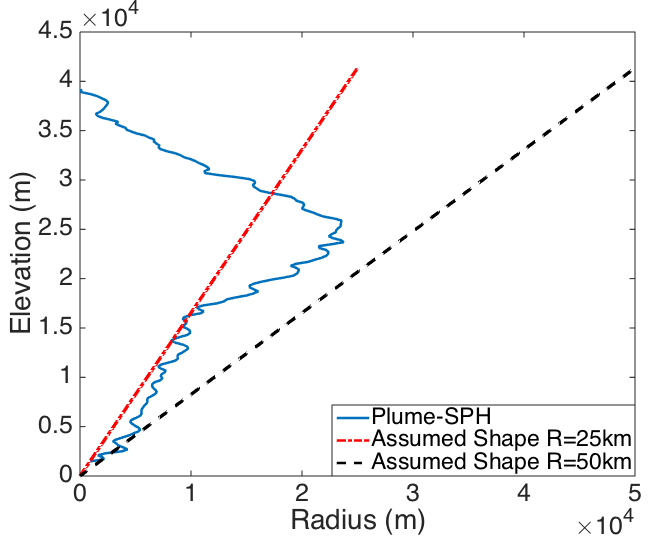
\includegraphics[width=0.50 \textwidth]{Figures/radius-Plume-SPH-And-Assumed}  
   \caption{Comparison between radius of initial ash clouds created by 3D plume model (Plume-SPH) and assumed initial ash cloud shape in Puff. The plume shape expression used in Puff defines an inverted cone whose actual shape changes when ``horizontal spread" takes different values. $R=25km$ is corresponding to ``horizontal spread" equals to $50km$. $R=50km$ is corresponding to ``horizontal spread" equals to $100km$}
    \label{fig:radius-comparison}
\end{figure}

Comparison between cross-sectional views of the initial ash clouds is shown in Fig. \ref{fig:initial-cloud-horizontal}. The cross-sectional view of assumed plume shape (last figure in Fig. \ref{fig:initial-cloud-horizontal}) is similar to cross-sectional view of simulated 3D plume in general sense. However, for simulated 3D plume, the ash particle distribution on cross section varies along with height. It is hard for semiempirical expressions to have such a distribution. In Puff, particle distribution on cross sections is assumed to be the same. 

\begin{figure}[!htb]
\centering
    \begin{minipage}{.325 \textwidth}
        \centering
        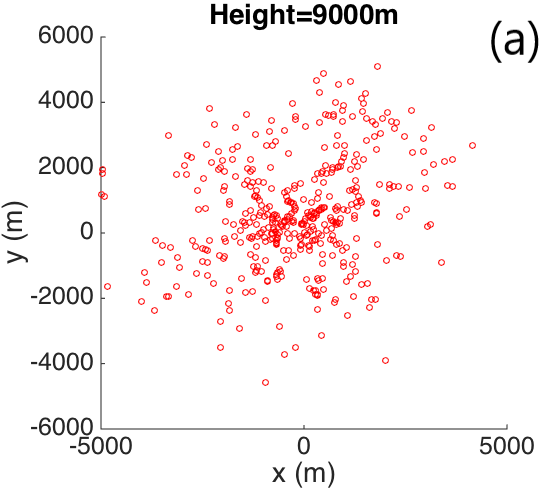
\includegraphics[width=0.99 \textwidth]{Figures/Possion-H9km-ParticleDis-h}
    \end{minipage}%
    \begin{minipage}{.325 \textwidth}
        \centering
        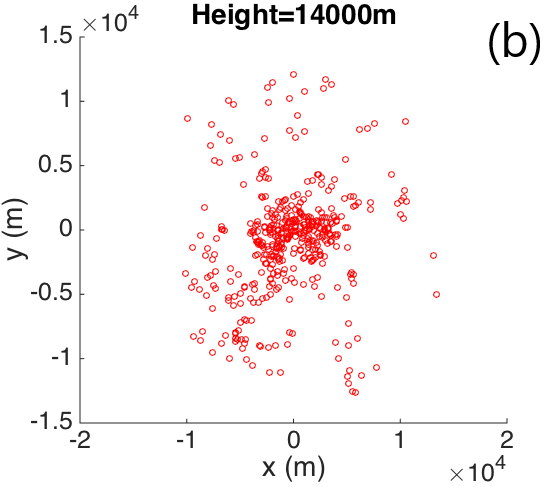
\includegraphics[width=0.99 \textwidth]{Figures/Possion-H14km-ParticleDis-h}
    \end{minipage}%  
    \begin{minipage}{.325 \textwidth}
        \centering
        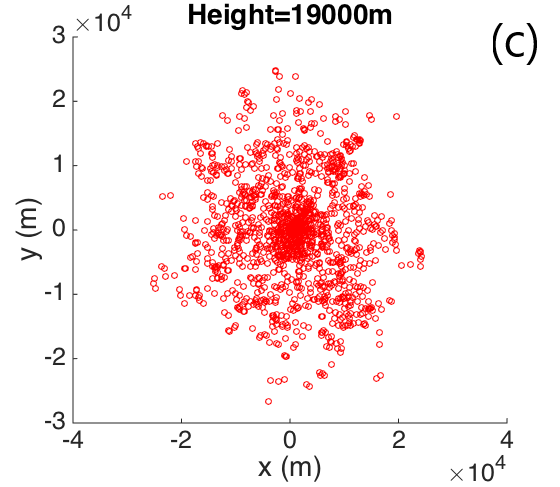
\includegraphics[width=0.99 \textwidth]{Figures/Possion-H19km-ParticleDis-h}
    \end{minipage}% 
    \\ 
    \begin{minipage}{.325 \textwidth}
        \centering
        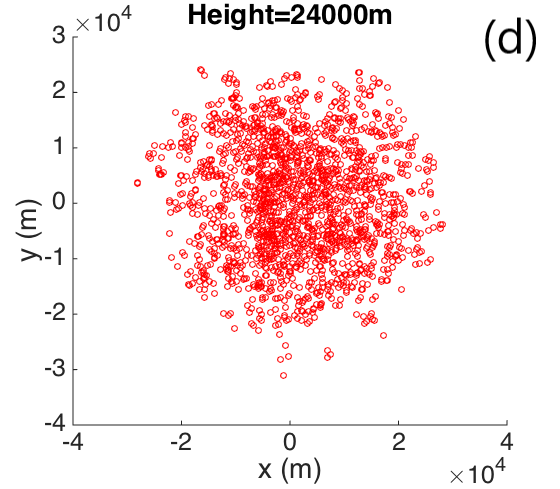
\includegraphics[width=0.99 \textwidth]{Figures/Possion-H24km-ParticleDis-h}
    \end{minipage}%
    \begin{minipage}{.325 \textwidth}
        \centering
        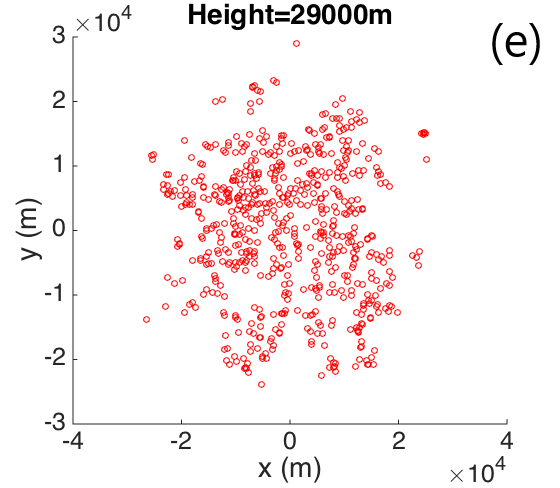
\includegraphics[width=0.99 \textwidth]{Figures/Possion-H29km-ParticleDis-h}
    \end{minipage}%  
    \begin{minipage}{.325 \textwidth}
        \centering
        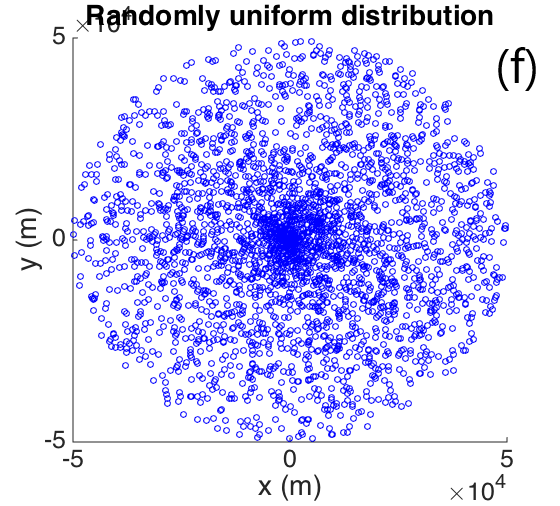
\includegraphics[width=0.99 \textwidth]{Figures/Possion-RDU-ParticleDis-h}
    \end{minipage}%  
    \caption{Horizontal distribution of ash particles (tracers) on a cross section of initial ash cloud. Puff assumes randomly uniform distribution of ash particle within a circle, as shown by blue dots in the last figure. All other figures show ash particle distribution of initial ash cloud created by Plume-SPH at different elevations.}
    \label{fig:initial-cloud-horizontal}
\end{figure}


Assigning different values to ``horizontal spread" has ignorable effect on VATD simulation results. We use numbers between $50 km$ to $1600 km$ as ``horizontal spread" to create initial ash cloud for VATD, all of them generate very similar results. Figure \ref{fig:ash-distribution-horizontal-compare} shows two different simulation results based on initial ash cloud with ``horizontal spread" equals to $50 km$ and $600 km$ respectively. No visible differences are apparent between them. This implies that horizontal distribution has less significant influence on VATD simulation results than vertical distribution.

\begin{figure}[!htb]
\centering
    \begin{minipage}{.325 \textwidth}
        \centering
        \includegraphics[width=0.99 \textwidth]{Figures/bent-55hr-ash-R25km}
    \end{minipage}%
    \begin{minipage}{.325 \textwidth}
        \centering
        \includegraphics[width=0.99 \textwidth]{Figures/bent-55hr-ash-R300km}
    \end{minipage}%  
    \caption{Ash transportation simulated by Puff at around 55 hours after eruption (UT 199106171141). Different values for ``horizontal spread" are used to create initial ash cloud. Pictures to the left is corresponding to ``horizontal spread" equals to $50 km m$. Pictures to the right is corresponding to ``horizontal spread" equals to $600 km m$. The observed cloud image is in Fig. \ref{fig:Plume-SPH-Puff-ash-cloud}.}
    \label{fig:ash-distribution-horizontal-compare}
\end{figure}

\section{Conclusion}

This paper presented, for the first time, VATD simulations using initial source conditions created by a 3D plume model.  Traditional VATD simulations use initial conditions created according to a semiempirical plume shape expression. A case study of the 1991 Pinatubo eruption demonstrates that a 3D plume model can create more realistic initial ash cloud and ash parcel positions, and therefore improve the accuracy of ash transport forecasts.  Informal sensitivity analyses suggest that initial conditions, as expressed in the disposition of initial ash parcel positions in the vertical, have a more significant effect on a volcanic ash transport forecast than most other parameters. Comparison of initial ash parcel distributions among the 3D plume model, semiempirical expressions, and observations suggests that a major subpopulation of ash parcels should be placed at a much lower elevation than maximum height to obtain a better VATD forecast. For the Pinatubo case study, ``well-matched'' simulation results are observed when using a maximum height of around $30 km$, which is much lower than the observed maximum height of $40 km$. Comparing the effects of the maximum height, vertical spread and horizontal spread shows that ash particle distribution in the vertical direction has the strongest effect on VATD simulation.

To summarize, we have presented a novel method for creating \textit{a priori} initial source conditions for VATD simulations. We have shown that it might be possible to obtain initial positions of ash parcels with deterministic forward modeling of the volcanic plume, obviating the need to attempt to obtain initial positions or a history of release heights via inversion \citep{stohl2011determination}. Although the method now suffers from the high computational cost associated with 3D forward modeling, it not only helps overcome shortcomings of existing methods used to generate \textit{a priori} input parameters, but also overcomes the need to do the thousands of runs associated with inverse modeling.  In addition, computational cost will continue to diminish as computing speed increases.  As they are forward numerical models based on first principles, 3D plume models need little if any parameterization, and user intervention should not be required to improve forecast power; no assumption about the initial position of ash parcels is needed. Generation of the initial cloud of ash parcels directly by 3D simulation is potentially adaptable to a variety of volcanic and atmospheric scenarios.  In contrast, semiempirical expressions used to determine initial conditions require several parameters to control ash particle distribution along a vertical line source or some simplified shape of the initial ash cloud, making it difficult in some cases to generate initial conditions that closely resemble a complex reality.

The full range of research issues raised by numerical forecasting of volcanic clouds is diverse. We described in this paper the effect of initial conditions chosen from the output of a 3D plume model on numerical forecasts of volcanic ash transport simulation.  The wind field, another important factor in volcanic ash transportation simulation is not discussed in the present work. Some other aspects, such as small scale physical processes, even though they play lesser roles, might need to be included in VATDs to improve accuracy for a particular eruption. In addition, eruption conditions are subject to change with time, even during the climactic phase of an eruption.  In the future, time-dependent initial conditions for VATDs can be created from 3D plume simulations with time-dependent eruption conditions.

%Text here ===>>>

%%

%  Numbered lines in equations:
%  To add line numbers to lines in equations,
%  \begin{linenomath*}
%  \begin{equation}
%  \end{equation}
%  \end{linenomath*}



%% Enter Figures and Tables near as possible to where they are first mentioned:
%
% DO NOT USE \psfrag or \subfigure commands.
%
% Figure captions go below the figure.
% Table titles go above tables;  other caption information
%  should be placed in last line of the table, using
% \multicolumn2l{$^a$ This is a table note.}
%
%----------------
% EXAMPLE FIGURE
%
% \begin{figure}[h]
% \centering
% when using pdflatex, use pdf file:
% \includegraphics[natwidth=800px,natheight=600px]{figsamp.pdf}
%
% when using dvips, use .eps file:
% \includegraphics[natwidth=800px,natheight=600px]{figsamp.eps}
%
% \caption{Short caption}
% \label{figone}
%  \end{figure}
%
% We recommend that you provide the native width and height (natwidth, natheight) of your figures.
% Specifying native dimensions ensures that your figures are properly scaled
%
%
% ---------------
% EXAMPLE TABLE
%
% \begin{table}
% \caption{Time of the Transition Between Phase 1 and Phase 2$^{a}$}
% \centering
% \begin{tabular}{l c}
% \hline
%  Run  & Time (min)  \\
% \hline
%   $l1$  & 260   \\
%   $l2$  & 300   \\
%   $l3$  & 340   \\
%   $h1$  & 270   \\
%   $h2$  & 250   \\
%   $h3$  & 380   \\
%   $r1$  & 370   \\
%   $r2$  & 390   \\
% \hline
% \multicolumn{2}{l}{$^{a}$Footnote text here.}
% \end{tabular}
% \end{table}

%% SIDEWAYS FIGURE and TABLE
% AGU prefers the use of {sidewaystable} over {landscapetable} as it causes fewer problems.
%
% \begin{sidewaysfigure}
% \includegraphics[width=20pc]{figsamp}
% \caption{caption here}
% \label{newfig}
% \end{sidewaysfigure}
%
%  \begin{sidewaystable}
%  \caption{Caption here}
% \label{tab:signif_gap_clos}
%  \begin{tabular}{ccc}
% one&two&three\\
% four&five&six
%  \end{tabular}
%  \end{sidewaystable}

%% If using numbered lines, please surround equations with \begin{linenomath*}...\end{linenomath*}
%\begin{linenomath*}
%\begin{equation}
%y|{f} \sim g(m, \sigma),
%\end{equation}
%\end{linenomath*}

%%% End of body of article

%%%%%%%%%%%%%%%%%%%%%%%%%%%%%%%%
%% Optional Appendix goes here
%
% The \appendix command resets counters and redefines section heads
%
% After typing \appendix
%
%\section{Here Is Appendix Title}
% will show
% A: Here Is Appendix Title
%
%\appendix
%\section{Here is a sample appendix}

%%%%%%%%%%%%%%%%%%%%%%%%%%%%%%%%%%%%%%%%%%%%%%%%%%%%%%%%%%%%%%%%
%
% Optional Glossary, Notation or Acronym section goes here:
%
%%%%%%%%%%%%%%
% Glossary is only allowed in Reviews of Geophysics
%  \begin{glossary}
%  \term{Term}
%   Term Definition here
%  \term{Term}
%   Term Definition here
%  \term{Term}
%   Term Definition here
%  \end{glossary}

%
%%%%%%%%%%%%%%
% Acronyms
%   \begin{acronyms}
%   \acro{Acronym}
%   Definition here
%   \acro{EMOS}
%   Ensemble model output statistics
%   \acro{ECMWF}
%   Centre for Medium-Range Weather Forecasts
%   \end{acronyms}

%
%%%%%%%%%%%%%%
%% Notation
%   \begin{notation}
%   \notation{$a+b$} Notation Definition here
%   \notation{$e=mc^2$}
%   Equation in German-born physicist Albert Einstein's theory of special
%  relativity that showed that the increased relativistic mass ($m$) of a
%  body comes from the energy of motion of the body—that is, its kinetic
%  energy ($E$)—divided by the speed of light squared ($c^2$).
%   \end{notation}




%%%%%%%%%%%%%%%%%%%%%%%%%%%%%%%%%%%%%%%%%%%%%%%%%%%%%%%%%%%%%%%%
%
%  ACKNOWLEDGMENTS
%
% The acknowledgments must list:
%
% >>>>	A statement that indicates to the reader where the data
% 	supporting the conclusions can be obtained (for example, in the
% 	references, tables, supporting information, and other databases).
%
% 	All funding sources related to this work from all authors
%
% 	Any real or perceived financial conflicts of interests for any
%	author
%
% 	Other affiliations for any author that may be perceived as
% 	having a conflict of interest with respect to the results of this
% 	paper.
%
%
% It is also the appropriate place to thank colleagues and other contributors.
% AGU does not normally allow dedications.


\acknowledgments
Support for the Twentieth Century Reanalysis Project dataset is provided by the U.S. Department of Energy, Office of Science Innovative and Novel Computational Impact on Theory and Experiment (DOE INCITE) program, and Office of Biological and Environmental Research (BER), and by the National Oceanic and Atmospheric Administration Climate Program Office.


%% ------------------------------------------------------------------------ %%
%% References and Citations

%%%%%%%%%%%%%%%%%%%%%%%%%%%%%%%%%%%%%%%%%%%%%%%
% BibTeX is preferred:
%
% \bibliography{<name of your .bib file>}
%
% don't specify bibliographystyle
%%%%%%%%%%%%%%%%%%%%%%%%%%%%%%%%%%%%%%%%%%%%%%%



% Please use ONLY \citet and \citep for reference citations.
% DO NOT use other cite commands (e.g., \cite, \citeyear, \nocite, \citealp, etc.).
%% Example \citet and \citep:
%  ...as shown by \citet{Boug10}, \citet{Buiz07}, \citet{Fra10},
%  \citet{Ghel00}, and \citet{Leit74}.

%  ...as shown by \citep{Boug10}, \citep{Buiz07}, \citep{Fra10},
%  \citep{Ghel00, Leit74}.

%  ...has been shown \citep [e.g.,][]{Boug10,Buiz07,Fra10}.


\bibliography{dissertation.bib}
\end{document}



%More Information and Advice:

%% ------------------------------------------------------------------------ %%
%
%  SECTION HEADS
%
%% ------------------------------------------------------------------------ %%

% Capitalize the first letter of each word (except for
% prepositions, conjunctions, and articles that are
% three or fewer letters).

% AGU follows standard outline style; therefore, there cannot be a section 1 without
% a section 2, or a section 2.3.1 without a section 2.3.2.
% Please make sure your section numbers are balanced.
% ---------------
% Level 1 head
%
% Use the \section{} command to identify level 1 heads;
% type the appropriate head wording between the curly
% brackets, as shown below.
%
%An example:
%\section{Level 1 Head: Introduction}
%
% ---------------
% Level 2 head
%
% Use the \subsection{} command to identify level 2 heads.
%An example:
%\subsection{Level 2 Head}
%
% ---------------
% Level 3 head
%
% Use the \subsubsection{} command to identify level 3 heads
%An example:
%\subsubsection{Level 3 Head}
%
%---------------
% Level 4 head
%
% Use the \subsubsubsection{} command to identify level 3 heads
% An example:
%\subsubsubsection{Level 4 Head} An example.
%
%% ------------------------------------------------------------------------ %%
%
%  IN-TEXT LISTS
%
%% ------------------------------------------------------------------------ %%
%
% Do not use bulleted lists; enumerated lists are okay.
% \begin{enumerate}
% \item
% \item
% \item
% \end{enumerate}
%
%% ------------------------------------------------------------------------ %%
%
%  EQUATIONS
%
%% ------------------------------------------------------------------------ %%

% Single-line equations are centered.
% Equation arrays will appear left-aligned.

%Math coded inside display math mode \[ ...\]
% will not be numbered, e.g.,:
% \[ x^2=y^2 + z^2\]
%
% Math coded inside \begin{equation} and \end{equation} will
% be automatically numbered, e.g.,:
% \begin{equation}
% x^2=y^2 + z^2
% \end{equation}


% To create multiline equations, use the
% \begin{eqnarray} and \end{eqnarray} environment
% as demonstrated below.
%\begin{eqnarray}
%  x_{1} & = & (x - x_{0}) \cos \Theta \nonumber \\
%        && + (y - y_{0}) \sin \Theta  \nonumber \\
%  y_{1} & = & -(x - x_{0}) \sin \Theta \nonumber \\
%        && + (y - y_{0}) \cos \Theta.
%\end{eqnarray}

%If you don't want an equation number, use the star form:
%\begin{eqnarray*}...\end{eqnarray*}

% Break each line at a sign of operation
% (+, -, etc.) if possible, with the sign of operation
% on the new line.

% Indent second and subsequent lines to align with
% the first character following the equal sign on the
% first line.

% Use an \hspace{} command to insert horizontal space
% into your equation if necessary. Place an appropriate
% unit of measure between the curly braces, e.g.
% \hspace{1in}; you may have to experiment to achieve
% the correct amount of space.


%% ------------------------------------------------------------------------ %%
%
%  EQUATION NUMBERING: COUNTER
%
%% ------------------------------------------------------------------------ %%

% You may change equation numbering by resetting
% the equation counter or by explicitly numbering
% an equation.

% To explicitly number an equation, type \eqnum{}
% (with the desired number between the brackets)
% after the \begin{equation} or \begin{eqnarray}
% command.  The \eqnum{} command will affect only
% the equation it appears with; LaTeX will number
% any equations appearing later in the manuscript
% according to the equation counter.
%

% If you have a multiline equation that needs only
% one equation number, use a \nonumber command in
% front of the double backslashes (\\) as shown in
% the multiline equation above.

% If you are using line numbers, remember to surround
% equations with \begin{linenomath*}...\end{linenomath*}

%  To add line numbers to lines in equations:
%  \begin{linenomath*}
%  \begin{equation}
%  \end{equation}
%  \end{linenomath*}



